\documentclass[a4paper,10pt]{book}
\usepackage[T1]{fontenc}
\usepackage[scaled]{luximono}
\usepackage[centertags]{amsmath}
%\usepackage{babel}
\usepackage{graphicx}
%\usepackage[applemac]{inputenc}
\usepackage{color}
\usepackage{colortbl}
\usepackage[colorlinks,urlcolor=blue]{hyperref}
\usepackage{fancybox,calc}
\usepackage{alltt}
\usepackage[Lenny]{fncychap}
\usepackage{makeidx}
\usepackage{fancyvrb}
\usepackage{listings}
\lstset{backgroundcolor=\color[gray]{0.8},language=Lisp,captionpos=b,showstringspaces=false,basicstyle=\ttfamily}
\usepackage{pifont}
\usepackage{lettrine}
\usepackage{soul}
\usepackage{appendix}
\usepackage{epigraph}
\usepackage{verbatim}
\usepackage[ruled,vlined,linesnumbered]{algorithm2e}
\usepackage{subfig}
\usepackage{commath}

%\renewcommand\lstlistingname{Listagem}

\bibliographystyle{plain}

\setlength\marginparwidth{80pt}

\newcommand\marginlabel[1]{\mbox{}\marginpar{\raggedright\hspace{0pt}\textcolor{blue}{#1}}}


\newcommand{\reguaH}[1]{\noindent \rule{\linewidth}{#1mm}}



  
%%%%%%%%%%%%%%%%
\begin{document}

\begin{titlepage}
%\pagecolor[rgb]{0.85,0.84,0.60}

\vspace*{3.5cm}
\begin{figure}[htbp] %  figure placement: here, top, bottom, or page
   \centering
   \includegraphics[scale=2.0]{capa/timbre.eps} 
\end{figure}

\vspace*{2.0cm}

\vspace*{\stretch{1}} \reguaH{1.5}
\begin{flushright}
\LARGE Evolutionary Computation\\{\color{red}{Course Notes}}\\
 \vspace*{2cm} Ernesto Costa 
\end{flushright}
\reguaH{1.5}


\begin{center}
\vspace*{\stretch{2}} Vers�o 0.01 
\date{\today}
\end{center}
\end{titlepage}

%\pagecolor{white}


\tableofcontents
\listoftables
\listoffigures

\chapter*{Preface}\label{cap:preface}


\epigraph{\ldots}{\ldots}


This a companion text for the course Evolutionary Computation of the Department of Informatics Engineering of the University of Coimbra. The course starts in 2006,  and we think it  is now time to compile the material presented to students in the form of simple notes. There are already some good general books on the subject of nature inspired computation (see \cite{Castro2006}, \cite{Floreano2008}, \cite{Brabazon2015}), so our aim is not to write another one. \\


\paragraph{Acknowledgments}.\\
\chapter{Introduction} \label{cap:int}

\section{Problem Solving and Computers}

\lettrine{W}{hen} you look around us we often ask ourselves one simple question: How such diverse and complex things did appear? Today we have a partial answer to this question.


\begin{comment}

\lettrine{Q}{uando} olhamos a nossa volta e vemos o que nos rodeia, incluindo
os nossos semelhantes, n�o podemos deixar de nos questionar:  como
foi poss�vel o aparecimento de tamanha complexidade e diversidade?
Qual a origem de tudo isto? Hoje temos respostas parciais para estas
quest�es. Achamos que o Universo � o resultado de um enorme Big
Bang, que a vida, baseada no carbono, surge da mat�ria como
resultado de reac��es qu�micas e que n�s, seres inteligentes somos a
fase superior de um processo evolutivo aberto que n�o p�ra.\\

Um dos aspectos que mais distingue os humanos � o seu desejo,
dir�amos compulsivo, de colocar quest�es e procurar respostas
\footnote{O mito de Pandora...}. Somos um agente resolvedor de
problemas \marginlabel{Agente Resolvedor de Problemas}. O
aparecimento do computador em meados do s�culo passado veio
amplificar a nossa capacidade de resolver em tempo �til os problemas mais diversos
e complexos. Dizemsos amplificar num duplo sentido: por um lado,
porque a sua rapidez nos torna a n�s humanos mais eficientes na obten��o de
respostas; mas, por outro lado, ao funcionar tamb�m ele pr�prio como
um processador de s�mbolos, o computador pode substituir-nos na resolu��o de
tarefas que se fossem executadas por n�s requeriam o uso da nossa
intelig�ncia. A �rea hoje conhecida por Intelig�ncia Artificial
\marginlabel{Intelig�ncia Artificial} (IA), tem por objecto a
resolu��o de forma aut�noma pela m�quina de problemas que exigem
intelig�ncia\footnote{A possibilidade dos computadores serem
inteligentes � um debate filos�fico interessante e que precedeu o
pr�prio aparecimento dos computadores. O teste de Turing � um
exemplo da tentativa de provar que as m�quinas n�o s�o diferentes,
no que respeita � intelig�ncia, dos seres humanos. Est� fora do
�mbito deste texto discutir esta quest�o}. Tradicionalmente a IA
procurou no ser humano o modelo, que depois de compreendido e
formalizado poderia ser incorporado nas m�quinas. N�o � este no
entanto o �nico caminho poss�vel e, por isso, durante os �ltimos
anos t�m aparecido met�foras alternativas � resolu��o inteligente de
problemas complexos. Neste texto tentaremos compreender
um desses caminhos alternativos.\\

Mat�ria, Vida e Consci�ncia s�o os tr�s grandes aspectos do mundo
que queremos entender. A eles se dedicaram ci�ncias como a F�sica, a
Biologia ou a Psicologia, com a Matem�tica sempre a servir de base
de apoio. N�o est�o isolados na medida que da mat�ria surgiu a vida,
e desta os seres conscientes. Est�o ligados como as c�lebres bonecas
russas conhecidas por Matrioskas (ver figura \ref{fig:matrioskas}).
Foi pois com naturalidade que, na egunda metade do s�culo passado, se come�ou a
equacionar a possibilidade de podermos explicar o que se passa em
cada um destes campos de observa��o por recurso aos mecanismos
utilizados nos outros dom�nios. Assim, por exemplo, aspectos de
auto-organiza��o que ocorrem na mat�ria tamb�m se manifestam em
agentes biol�gicos; os mecanismos evolutivos dos seres vivos
permitem-nos entender melhor o aparecimento da linguagem e os seus
mecanismos.\\


\begin{figure}[!h]
  \centering
  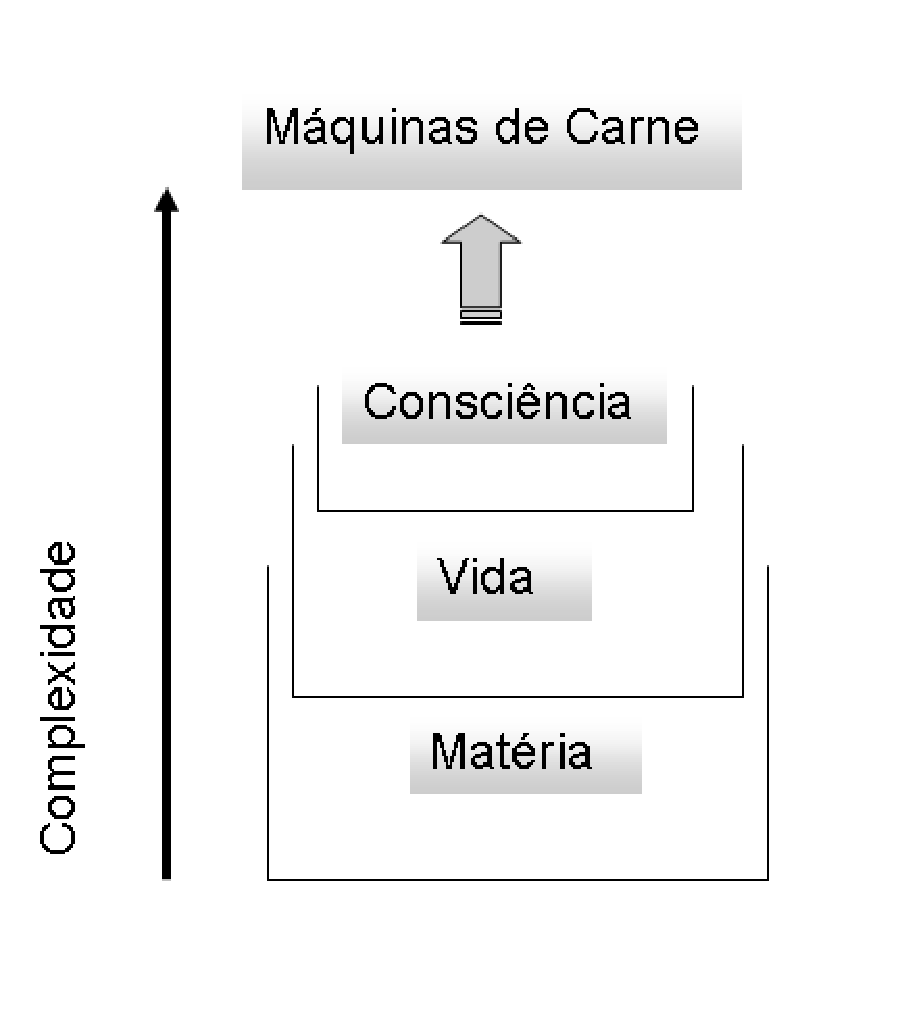
\includegraphics[scale=0.4]{cap01/matrioskas.eps}\\
  \caption{Mat�ria, Vida e Consci�ncia}\label{fig:matrioskas}
\end{figure}


N�s queremos desenvolver essa ideia de um modo muito preciso: em que
medida mecanismos e processos que ocorrem nos seres vivos
(individualmente, como esp�cie ou como sociedades organizadas), e de um modo mais geral  na natureza, nos
podem ajudar a resolver computacionalmente problemas complexos. Ao corpo de conhecimento pr�tico e te�rico que tem vindo a ser constru�do  chamamos de Computa��o Inspirada na Natureza (CIN))\marginlabel{Computa��o Inspirada na Natureza}.



\section{As diferentes perspectivas} \label{sec:perspec}

\lettrine{D}{issemos} na sec��o anterior que uma entidade viva pode ser vista
pelo menos de tr�s perspectivas diferentes:

\begin{itemize}
    \item como um entidade isolada
    \item como um membro de uma esp�cie
    \item com um elemento de uma sociedade
\end{itemize}

Cada uma destas vistas tem sido objecto de estudo: podemos estar
interessados em compreender o funcionamento do sistema imune nos
mam�feros, podemos tentar entender como as esp�cies t�m evolu�do ao
longo do tempo, podemos, finalmente estar interessados em entender a
forma��o de colectivos de indiv�duos todos eles sujeitos a um
conjunto de regras comportamentais. A Computa��o Inspirada na Natureza prop�e novos modelos, baseados nalguns destes mecanismos e processos, que podem ser transportados e
operacionalizados numa m�quina. Ao longo do tempo foram-se
sedimentando novas �reas que d�o corpo � CIN \footnote{Os temas
apresentados n�o s�o exaustivos. Ficaram de fora aspectos como as
redes neuronais, os computadores baseados em DNA ou ainda os
Imunocomputadores} (ver figura \ref{fig:cib}).

\begin{figure}[!h]
  \centering
  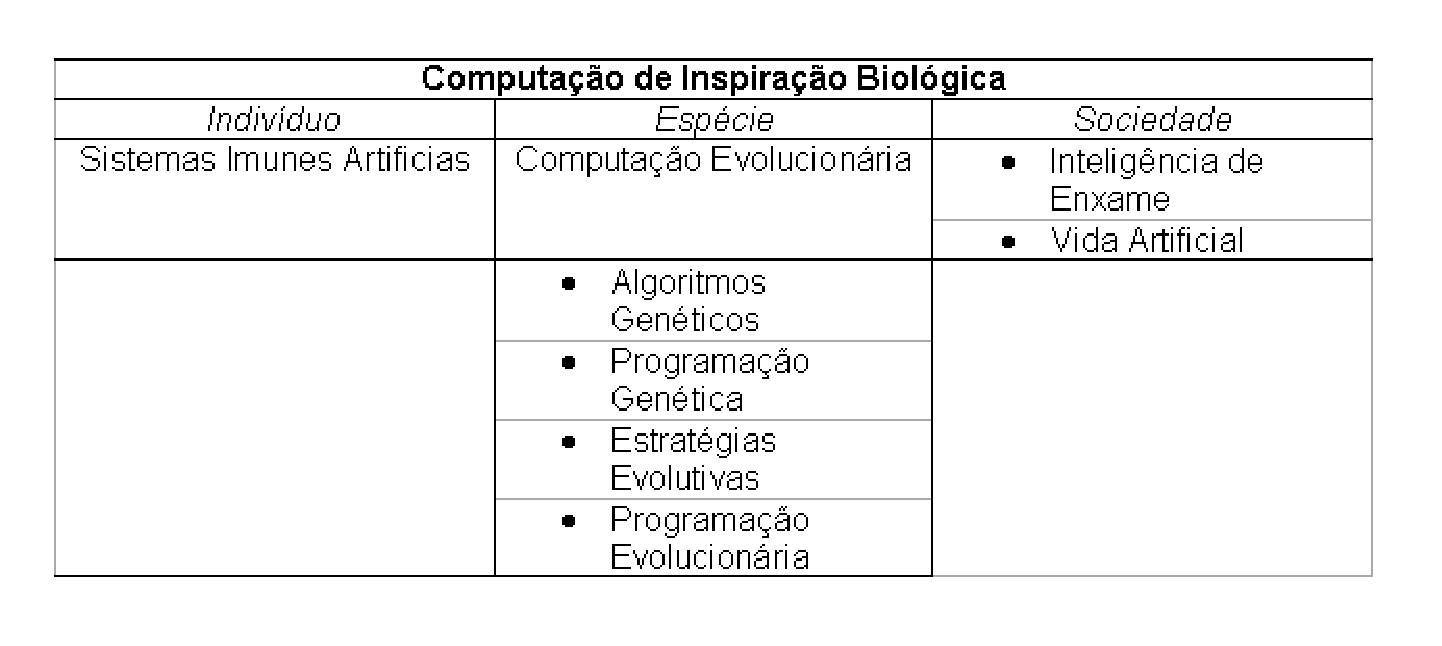
\includegraphics[scale=0.5]{intro/cib.eps}\\
  \caption{CIN: as diferentes �reas}\label{fig:cib}
\end{figure}

Os Sistemas Imunes Artificias \marginlabel{Sistemas Imunes
Artificiais}, como o seu nome indica, baseiam-se no sistema imune
dos mam�feros, dele retendo princ�pios que descrevem as interac��es
entre os agentes patog�nicos e os anticorpos. Esses princ�pios s�o
usados para resolver os mais diversos problemas desde a detec��o de
intrus�o em redes inform�ticas at� � previs�o da
estrutura 3D de prote�nas.\\

A Computa��o Evolucion�ria \marginlabel{Computa��o Evolucion�ria}
procura aplicar os mecanismos da selec��o natural de Darwin e da
gen�tica de Mendel, para melhor resolver problemas em particular de
optimiza��o que, ou n�o t�m solu��o anal�tica ou essa solu��o
anal�tica n�o � comput�vel em tempo �til. Problemas como o caminho
mais curto num grafo ou o projecto da estrutura de turbinas s�o
exemplos de problemas concretos que esta abordagem permite resolver
satisfatoriamente. Por raz�es hist�rias esta abordagem deu origem a
quatro subfam�lias
que ser�o estudadas com detalhe no cap�tulo \ref{cap:ce}.\\

A Intelig�ncia de Enxame \marginlabel{Intelig�ncia de Enxame}
inspira-se no comportamento de algumas sociedades de seres vivos,
como as formigas ou as vespas, para da� derivar solu��es para
problemas como seja optimizar a comunica��o entre computadores ou
manter um conjunto de micro-sat�lites em forma��o no espa�o.

A Vida Artificial \marginlabel{Vida Artificial} pretende, no dizer
do seu fundador Christopher Langton, "estudar a vida como poderia
ter sido", e tem permitido encontrar respostas a quest�es como a
emerg�ncia de padr�es est�veis por interac��o simples entre unidades
elementares \footnote{Em todo o rigor, a �rea da Vida Artificial
mais do que relevar da computa��o com inspira��o biol�gica pode ser
vista antes como a Biologia como computa��o}.

\section{Os objectivos do texto}

\lettrine{E}{ste} texto tem como �nica pretens�o ser uma breve introdu��o �
Computa��o Inspirada na Natureza. Deste modo ser�o apresentados
nos pr�ximos cap�tulos as sete componentes mencionadas na sec��o
\ref{sec:perspec}. Para cada abordagem enunciaremos os princ�pios,
apresentaremos exemplos e chamaremos a aten��o para alargamentos
poss�veis e para problemas ainda por resolver de modo satisfat�rio.
Colocaremos no final alguns problemas e desafios e explicitaremos
bibliografia relevante.\\

Um aspecto que tamb�m trataremos � o da nova �rea conhecida por
Bioinform�tica \marginlabel{Bioinform�tica}. Em particular,
debru�ar-nos-emos sobre a forma como a CIN pode ela pr�pria "pagar
de volta" � Biologia fornecendo-lhe novas solu��es para quest�es
antigas, como o alinhamento de sequ�ncias ou o problema do
enrolamento tridimensional de prote�nas.\\

O leitor interessado em aprofundar os seus conhecimentos pode
consultar as obras \cite{costa2004}, \cite{eiben2003},
\cite{castro2002} e \cite{fogel2003}.

\end{comment}


\chapter{Gradient-Based Optimization}\label{cap:gradient}

\section{Introduction}

\section{Algorithms}

\subsection{Gradient Ascendent} 

This is the most simple algorithm to find the maximum of a function, as discussed in class (see the algorithm \ref{alg:gasc}). It is based on the idea of, starting at a random point,  iteratively improving the result by following the direction  of the gradient of the function (i.e., the derivative).

\begin{algorithm}
\SetKwData{Assign}{$\leftarrow$}
\SetKwInOut{Input}{Input}
\SetKwInOut{Output}{Output}

\caption{{\bf Gradient Ascendent\label{alg:gasc}}}
\BlankLine
\Input{Problem,$ \nabla f$, $\alpha$}
\Output{Best}
\BlankLine

\DataSty{Best} \Assign \FuncSty{RandomSolution}(Problem)

\Repeat{ found ideal solution or run out of time}
{\DataSty{Best} \Assign  \DataSty{Best} +  $\alpha \nabla$ f(\DataSty{Best})}


\KwRet{\DataSty{Best}}

\end{algorithm}

The operator $\nabla f$ computes the vector of the derivatives for each dimension. In the unidimensional case it is just $\od{f}{x}$. The way it is defined, the algorithm try to find out the \textbf{maximum} of the function. If we want the \textbf{minimum} we just have to change the add operation to a minus in the update (line 3 of the pseudo code), and we do a gradient descent algorithm. The reason why we do so is related with the sign of the derivative. In fact, if the derivative at a point is negative and we are maximizing,  the value of $x$ must be reduced, while if we are minimizing that value must be increased. The same reasoning applies when the derivative is positive (see figure \ref{fig:grad1}). 

\begin{figure}[!htbp] 
   \begin{center}
   \includegraphics[scale=0.5]{cap02/imagens/grad.png} 
   \caption{When the derivative is positive (at $x_1$) the new value for $x$ must be greater if we are maximizing, smaller if we are minimizing. When the derivative is negative (at $x_2$) the new value for $x$ must be lower if we are maximizing, greater if we are minimizing.}
   \label{fig:grad1}
   \end{center}
\end{figure}



\subsection{Random Restart} 

This algorithm apply the same idea but with random restart. Algorithm \ref{alg:rnd} show the pseudo-code. As expected we now have two cycles. The external one controls how many times we perform a gradient ascendent. The idea is that trying different starting points $x$ we can avoid being trapped in a local maximum. 



\begin{algorithm}
\SetKwData{Assign}{$\leftarrow$}
\SetKwInOut{Input}{Input}
\SetKwInOut{Output}{Output}

\caption{{\bf Gradient Ascendent with random restart\label{alg:rnd}}}
\BlankLine
\Input{Problem, $f$, $ \nabla f$, $\alpha$}
\Output{Best}
\BlankLine

\DataSty{x} \Assign \FuncSty{RandomSolution}(Problem) \;
\DataSty{Best} \Assign \DataSty{x}

\Repeat{ found ideal solution or run out of time}
{
\Repeat 
	{ $|| \nabla f(\DataSty{x}) || = 0$} 
	{\DataSty{\DataSty{x}} \Assign  \DataSty{\DataSty{x}} +  $\alpha \nabla$ f(\DataSty{\DataSty{x}})}
	
\If {$f(\DataSty{x}) \ge f(\DataSty{Best})$}{ \DataSty{Best} \Assign \DataSty{x}} 

x \Assign  \FuncSty{RandomSolution}(Problem)

}

\KwRet{\DataSty{Best}}

\end{algorithm}

It should be notice here that you are not going to find a point where the derivative is \textbf{exactly} equal to zero. So you have to define an $\epsilon$ such that if $ |f'(x)| < \epsilon$ you assume the derivative is zero.


\subsection{Newton's Method}

\section{Implementation}

The implementation of these methods in Python is straightforward, in particularly for the one dimensional case.  As they are based in the idea of using the derivative (first and second) we start with a small program to compute it.  You are free to implement your own solution!

\begin{lstlisting}
def derivative(f, delta_x=0.000001):
    """Return the derivative of a function"""
    def der(x):
        return (f(x+ delta_x) - f(x)) / delta_x
    return der
\end{lstlisting}

If we want to visualize the functions, the derivatives and the evolution of the best solution over time, we also need some code.

\begin{lstlisting}
import matplotlib.pyplot as plt

def display_function(f, x_min, x_max, delta=0.1):
    x = list(frange(x_min, x_max,delta))
    y = [f(i) for i in x]
    plt.title(f.__name__)
    plt.grid(True)
    plt.axhline(c='black')
    plt.axvline(c='black')    
    plt.xlabel('X')
    plt.ylabel('Y= '+f.__name__ + '(X)')
    plt.plot(x,y, 'r')
    plt.show()
\end{lstlisting}

\paragraph{frange}Notice the use of a function (\texttt{frange}, equivalent to  \texttt{range} but that works with floats. As there is not such a thing in Python\footnote{If you are using Python arrays this is not true, for we have the \texttt{arange} method in the \texttt{numpy} module.}, let's implement it too.

\begin{lstlisting}
def frange(n1,n2=None,n3=1.0):
    """
    Range with floats.
    Can be called as  with range:
    frange(n)
    frange(n1,n2)
    fange(n1,n2,n3)
    """
    if n2 == None:
        n2 = n1
        n1 = 0.0
    nextn = n1
    while (n3 >= 0.0 and nextn <= n2) or (n3 < 0.0 and nextn >= n2):
        yield nextn
        nextn += n3
\end{lstlisting}


-- INCLUDE: code for the evolution of the best solution...\\


\section{Exercices}
\chapter{Single-State Stochastic Search}\label{cap:single}

\section{Introduction}


\section{Algorithms}

\section{Implementation}

\section{Exercices}


%\include{c04/capitulo04}
%\include{c05/capitulo05}
%\include{c06/capitulo06}
%\include{c07/capitulo07}
%\include{c08/capitulo08}
%\include{c09/capitulo09}
%\include{c10/capitulo10}
%\include{c11/capitulo11}






\newpage

\appendix

%\include{A/anexoA}

%%%%%%%%%%%%%%%%%%%%%%%%%%%%%%%%%%%%%%%%%%%%%%%%%%%%%%%%%%%%%%%%%%%%%%%%%%%%%%%%%%%%
%
% Bibliografia
%
%%%%%%%%%%%%%%%%%%%%%%%%%%%%%%%%%%%%%%%%%%%%%%%%%%%%%%%%%%%%%%%%%%%%%%%%%%%%%%%%%
\newpage

\bibliography{cevol.bib}





\end{document}